\documentclass[a4paper,12pt]{article}

\usepackage[utf8]{inputenc}
%\usepackage[spanish]{babel}
\usepackage{exerlist}
\usepackage{math2}
\usepackage{amsmath}
\usepackage{tikz}
%\usetikzlibrary{babel}

\newcommand{\myneg}{\raise.17ex\hbox{$\scriptstyle\sim$}}%
\newcommand{\mysmallneg}{\raise.17ex\hbox{$\scriptscriptstyle\sim$}}%
\newcommand{\codlength}[1]{\left< #1 \right>}
\newcommand{\colvector}[1]{\left(\begin{array}{c} #1 \end{array}\right)}
\newcommand{\lineal}[1]{\mbox{lin}(#1)}
\newcommand{\Ppolar}[1]{#1^{\bigtriangleup}}
\renewcommand{\conv}[1]{\mathrm{conv}(#1)}
\renewcommand{\cone}[1]{\mathrm{cone}(#1)}

\setlecture{Geometría Discreta}
\setprofesor{Luis M. Torres}
\setexamdate{Mayo, 2026}

\begin{document}
\exercisetitle{Ejercicios guiados}

\noindent\textbf{Combinaciones lineales, afines, cónicas y convexas}

\begin{exerciselist}

    \item Considere la ecuación
    \[
        3x_1 + 2x_2 + x_3 = 0.
    \]
    Demuestre que toda combinación lineal de dos soluciones de esta ecuación es nuevamente una solución.

    \item Encuentre dos vectores \(x,y \in \mathbb{R}^3\) tales que toda solución de la ecuación del ejercicio anterior pueda escribirse como combinación lineal de \(x\) e \(y\).

    \item Sea \(A \in \mathbb{R}^{m \times d}\). Considere el sistema homogéneo
    \[
        Ax = 0.
    \]
    Demuestre que toda combinación lineal de dos soluciones del sistema es nuevamente una solución.

    \item En el contexto del ejercicio anterior, ¿existe un conjunto finito de vectores de \(\mathbb{R}^d\) tal que toda solución del sistema pueda escribirse como combinación lineal de dichos vectores? Justifique su respuesta.

    \item Considere ahora el siguiente sistema no homogéneo:
    \[
    \begin{cases}
        x_1 + x_2 - x_3 = 1, \\
        -x_1 + x_2 - x_3 = -1.
    \end{cases}
    \]
    Demuestre, mediante un contraejemplo, que una combinación lineal de dos soluciones del sistema no necesariamente es una solución.

    \item Dados \(x,y \in \mathbb{R}^d\), definimos una \emph{combinación afín} de \(x\) e \(y\) como un vector de la forma
    \[
        z = \alpha x + \beta y,
    \]
    donde \(\alpha,\beta \in \mathbb{R}\) satisfacen
    \[
        \alpha + \beta = 1.
    \]
    Demuestre que toda combinación afín de dos soluciones del sistema del ejercicio anterior es nuevamente una solución.

    \item Encuentre dos vectores de \(\mathbb{R}^3\) tales que toda solución del sistema del ejercicio 5 pueda escribirse como combinación afín de dichos vectores.

    \item Sean \(A \in \mathbb{R}^{m \times d}\) y \(b \in \mathbb{R}^m\). Considere el sistema no homogéneo
    \[
        Ax = b.
    \]
    Demuestre que toda combinación afín de dos soluciones del sistema es nuevamente una solución.

    \item En el contexto del ejercicio anterior, ¿existe un conjunto finito de vectores de \(\mathbb{R}^d\) tal que toda solución del sistema pueda escribirse como combinación afín de dichos vectores? Justifique su respuesta.
    
    \item Considerar $k+1$ puntos $x_0, x_1, \ldots, x_k \in \mathbb{R}^d$. Demuestre que $x \in \mathbb{R}^d$ es una combinación afín de estos puntos si, y solo si, $x - x_0$ puede escribirse como combinación lineal de los $k$ vectores $x_1 - x_0, x_2 - x_0, \ldots, x_k - x_0$.
    
    \item Considere el siguiente sistema de desigualdades en \(\mathbb{R}^2\):
    \[
    \begin{cases}
        -x_1 + 2x_2 \geq 0, \\
        x_1 + x_2 \geq 0.
    \end{cases}
    \]
    Demuestre, mediante un contraejemplo, que una combinación afín de dos soluciones del sistema no necesariamente es una solución.

    \item Dados \(x,y \in \mathbb{R}^d\), definimos una \emph{combinación cónica} (o \emph{cónica-convexa}) de \(x\) e \(y\) como un vector de la forma
    \[
        z = \alpha x + \beta y,
    \]
    donde \(\alpha,\beta \in \mathbb{R}\) satisfacen
    \[
        \alpha \geq 0,
        \qquad
        \beta \geq 0.
    \]
    Demuestre que toda combinación cónica de dos soluciones del sistema del ejercicio anterior es nuevamente una solución.

    \item Sea \(A \in \mathbb{R}^{m \times d}\). Considere el sistema homogéneo de desigualdades
    \[
        Ax \leq 0.
    \]
    Demuestre que toda combinación cónica de dos soluciones del sistema es nuevamente una solución.

    \item ¿Existe un conjunto finito de vectores de \(\mathbb{R}^2\) tal que toda solución del sistema del ejercicio 10 pueda escribirse como combinación cónica de dichos vectores? Justifique su respuesta.

\paragraph{Propuesta de solución.}

Sean
\[
v_1=(2,1),
\qquad
v_2=(-1,1).
\]

Observemos primero que ambos vectores satisfacen el sistema:
\[
\begin{cases}
-x_1+2x_2\geq 0,\\
x_1+x_2\geq 0.
\end{cases}
\]

Además, si \(\alpha,\beta\geq 0\), entonces
\[
x=\alpha v_1+\beta v_2 = (2\alpha-\beta,\alpha+\beta)
\]
satisface ambas desigualdades:
\[
-(2\alpha-\beta) + 2(\alpha+\beta) = 3\beta \geq 0,
\qquad
(2\alpha-\beta) + (\alpha+\beta) = 3\alpha \geq 0 .
\]

Recíprocamente, sea \(x=(x_1,x_2)\) una solución del sistema. Definimos
\[
\alpha=\frac{x_1+x_2}{3},
\qquad
\beta=\frac{2x_2-x_1}{3}.
\]

Como \(x\) satisface las desigualdades,
\[
x_1+x_2\geq 0,
\qquad
2x_2-x_1\geq 0,
\]
se tiene que \(\alpha,\beta\geq 0\).

Finalmente,
\[
\alpha(2,1)+\beta(-1,1)
=
(2\alpha-\beta,\alpha+\beta)
=
(x_1,x_2).
\]

Por lo tanto, toda solución del sistema puede escribirse como combinación cónica de los vectores
\[
(2,1)
\quad\text{y}\quad
(-1,1).
\]

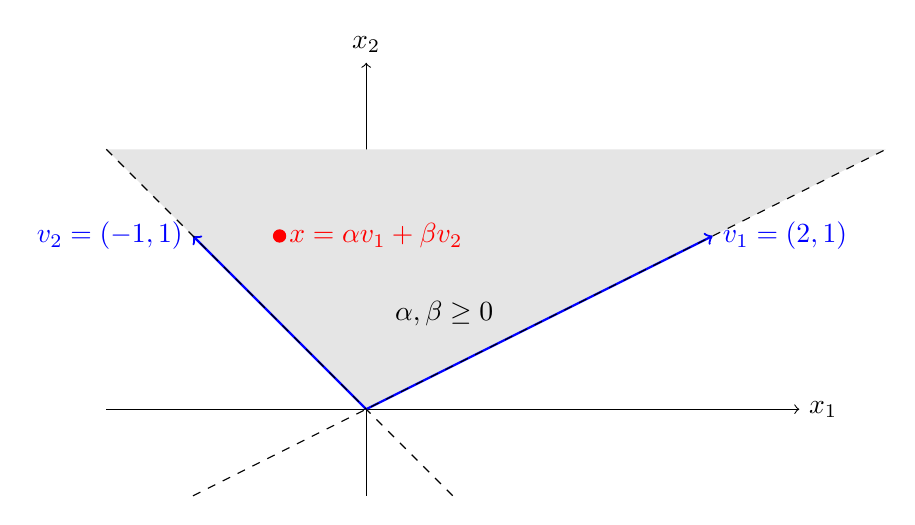
\begin{tikzpicture}[scale=1.1]

    % Ejes
    \draw[->] (-3,0) -- (5,0) node[right] {$x_1$};
    \draw[->] (0,-1) -- (0,4) node[above] {$x_2$};

    % Región del cono
    \fill[gray!20]
        (0,0) -- (6,3) -- (-3,3) -- cycle;

    % Rayos extremos
    \draw[thick,blue,->] (0,0) -- (4,2)
        node[right] {$v_1=(2,1)$};

    \draw[thick,blue,->] (0,0) -- (-2,2)
        node[left] {$v_2=(-1,1)$};

    % Rectas frontera
    \draw[dashed] (-3,3) -- (1,-1);
    \draw[dashed] (-2,-1) -- (6,3);

    % Punto interior
    \filldraw[red] (-1,2) circle (2pt)
        node[right] {$x=\alpha v_1+\beta v_2$};

    % Etiqueta
    \node at (0.9,1.1) {$\alpha,\beta\geq 0$};

\end{tikzpicture}

\item Un conjunto \(C \subset \mathbb{R}^d\) se llama \emph{cono} si, para todo \(x \in C\) y todo \(\alpha \geq 0\), se tiene
\[
\alpha x \in C.
\]

Por otro lado, un conjunto \(C \subset \mathbb{R}^d\) se llama \emph{convexo} si, para todo \(x,y \in C\) y todo \(\alpha,\beta \geq 0\) tales que
\[
\alpha+\beta=1,
\]
se tiene
\[
\alpha x+\beta y \in C.
\]

Demuestre que un conjunto \(C \subset \mathbb{R}^d\) es un cono convexo si, y solo si, para todo \(x,y \in C\) y todo \(\alpha,\beta \geq 0\), se cumple que
\[
\alpha x+\beta y \in C.
\]

Concluya que el conjunto de soluciones de un sistema homogéneo de desigualdades lineales es un cono convexo.

\item Demuestre que la intersección de una familia finita de conos convexos es nuevamente un cono convexo.

Concluya que, dado un conjunto \(S \subset \mathbb{R}^d\), existe un único cono convexo minimal que contiene a \(S\).

\item Dado un conjunto \(K \subset \mathbb{R}^d\), definimos la \emph{envolvente cónica} de \(K\) como la intersección de todos los conos convexos que contienen a \(K\). Denotaremos este conjunto por
\[
\cone{K}.
\]

Demuestre que si \(y_1,\dots,y_k \in K\) y \(t_1,\dots,t_k \in \mathbb{R}_+\), entonces
\[
t_1 y_1+\cdots+t_k y_k \in \cone{K}.
\]

\item Sean \(A \in \mathbb{R}^{m\times d}\) y \(b \in \mathbb{R}^m\). Considere el sistema no homogéneo de desigualdades
\[
Ax \leq b.
\]

Demuestre que el conjunto de soluciones del sistema es un conjunto convexo de \(\mathbb{R}^d\).

\item Demuestre que la intersección de una familia finita de conjuntos convexos es nuevamente un conjunto convexo.

Concluya que, dado un conjunto \(K \subset \mathbb{R}^d\), existe un único conjunto convexo minimal que contiene a \(K\). Denominaremos a este conjunto la \emph{envolvente convexa} de \(K\), y lo denotaremos por
\[
\conv{K}.
\]

\item Demuestre que si \(x_1,\dots,x_n \in K\) y \(\lambda_1,\dots,\lambda_n \in \mathbb{R}_+\) satisfacen
\[
\lambda_1+\cdots+\lambda_n=1,
\]
entonces
\[
\lambda_1x_1+\cdots+\lambda_nx_n \in \conv{K}.
\]

\end{exerciselist}

\noindent\textbf{Ejemplos de polítopos}

\begin{exerciselist}

\item Sean $V_1 = \{(0,0),(1,0),(0,1)\}$ y $V_2 = \{(0,2),(1,1),(2,0)\}$. Determine qué polítopos se obtienen como $\conv{V_1}$ y $\conv{V_2}$, y cuáles son sus dimensiones.

\item ¿Qué polítopos pueden obtenerse como envolventes convexas de 4 puntos?

\item ¿Cuál es la menor cantidad de puntos necesarios para generar un polítopo de dimensión $n$?

\item Sean $e_1,\dots,e_d$ los vectores canónicos de $\mathbb{R}^d$. Determine qué polítopo se obtiene como $\conv{\{e_1,\dots,e_d\}}$ y cuál es su dimensión.

\item Determine qué polítopo se obtiene como $\conv{\{0, e_1,\dots,e_d\}}$ y cuál es su dimensión.

\item Determine qué polítopo se obtiene en $\mathbb{R}^3$ como $\conv{\{e_1, -e_1, e_2, -e_2, e_3, -e_3\}}$ y cuál es su dimensión.

\item Sea $V = \{\sum_{i=1}^{3} \alpha_i e_i : \alpha_i \in \{-1,1\}, 1 \leq i \leq 3\}$. Determine qué polítopo se obtiene como $\conv{V}$ y cuál es su dimensión.

\item Partiendo de un segmento, ¿qué polítopos se obtienen al aplicar sucesivamente la operación de construir una pirámide?

\item Partiendo de un segmento, ¿qué polítopos se obtienen al aplicar sucesivamente la operación de construir una bipirámide?

\item Partiendo de un segmento, ¿qué polítopos se obtienen al aplicar sucesivamente la operación de construir un prisma?
\item Sean $V = \{ x_1, \ldots, x_n \} \subset \mathbb{R}^d$ y $P=\conv{V}$. Dados $a \in \mathbb{R}^d$ y $c \in \mathbb{R}$, se define el subconjunto $S$ de $V$ como
\[
S = \{ v \in V : a^T v = c \}.
\]
Demuestre que $\conv{S}$ es una cara de $P$ si y solamente si $a^T v - c$ tiene el mismo signo para todo $v \in V\setminus S$.
\item Sea $V = \{ x_1, \ldots, x_n \}$ un conjunto finito de puntos en $\mathbb{R}^d$ tal que ningún punto está en la envolvente convexa de los demás. Suponer que $P=\conv{V}$ es un polítopo simplicial, con $\dim(P)=d$. Sea $S \subset V$ un subconjunto de $V$ tal que $|S|=d$ y $\dim(\text{aff}(S))=d-1$.
\begin{exerciselist}
\item Demostrar que existe una función afín $F_S : \mathbb{R}^d \to \mathbb{R}$ tal que $F_S(x)=0$ para todo $x \in S$.
\item Demostrar que $\conv{S}$ es una faceta de $P$ si y solamente si y $F_S(x)$ tiene el mismo signo para todo $x \in V\setminus S$.
\end{exerciselist}
\end{exerciselist}

\noindent\textbf{Poliedros y optimización lineal}
\begin{exerciselist}
\item Sean $V= \{ x_1, \ldots, x_n \} \subset \mathbb{R}^d$, $P=\conv{V}$ y $c \in \mathbb{R}^d$. Demostrar que
$$
\max \{ c^T x : x \in P \} = \max \{ c^T x : x \in V \}.
$$
\item Sean $V= \{ x_1, \ldots, x_n \} \subset \mathbb{R}^d$, $Y= \{ y_1, \ldots, y_k \} \subset \mathbb{R}^d$, y $c \in \mathbb{R}^d$. Definimos:
$$
P = \{ x + y : x \in \conv{V}, y \in \cone{Y} \}.
$$
Demostrar que
\begin{exerciselist}
\item Si existe $y \in Y$ tal que $c^T y > 0$, entonces para todo $\alpha \in \mathbb{R}$, existe $x \in P$ tal que $c^T x > \alpha$, lo que implica que $\max \{ c^T x : x \in P \} = +\infty$.
\item Si $c^T y \leq 0$ para todo $y \in Y$, entonces
$$
\max \{ c^T x : x \in P \} = \max \{ c^T x : x \in V\}.
$$
\end{exerciselist}
\end{exerciselist}

\noindent\textbf{Teorema de Minkowski-Weyl}
\begin{exerciselist}
    \item Sean $A \in \mathbb{R}^{m \times d}$, $b \in \mathbb{R}^m$ y $P = \{ x \in \mathbb{R}^d : Ax \leq b \}$. Definimos
    \[
    C(P) = \left\{ {x_0 \choose x} \in \mathbb{R}^{d+1} : -x_0 b + A x \leq 0 \right\}.
    \]
    Demostrar que 
    $$
    P = \left\{ x \in \mathbb{R}^d : {1 \choose x} \in C(P) \right\}.
    $$
    \item Sean $V \in \mathbb{R}^{d \times n}$, $Y \in \mathbb{R}^{d \times k}$ y $P = \conv{V} + \cone{Y}$. Definimos
    \[
    C(P) = \textrm{cone}\left(\begin{array}{cc}
        \mathbf{1}^T & \mathbf{0}^T\\
        V & Y
    \end{array}\right),
    \]
    con $\mathbf{1} \in \mathbb{R}^n$ y $\mathbf{0} \in \mathbb{R}^k$. Demostrar que 
    $$
    P = \left\{ x \in \mathbb{R}^d : {1 \choose x} \in C(P) \right\}.
    $$
\item Sea $I \in \mathbb{d \times d}$ la matriz identidad. Demostrar que el conjunto
$$
C = \{ x \in \mathbb{R}^d : -I x \leq 0 \}
$$
es la envolvente cónica de un conjunto finito de vectores.

\item Sea $A \in \mathbb{R}^{m \times d}$. Demostrar que
$$
\{ Ax  : x \in \mathbb{R}^d \} = \cone{Y},
$$
donde 
$$
Y = \{Ae_i : 1 \leq i \leq d\} \cup \{-Ae_i : 1 \leq i \leq d\}.
$$ 

\item Sea $A \in \mathbb{R}^{m \times d}$. Demostrar que
$$
\left\{ {x \choose w} \in \mathbb{R}^{d+m} : A x \leq w \right\} = \cone{Y},
$$
donde 
$$
Y = \left\{{e_i \choose Ae_i} : 1 \leq i \leq d\right\} \cup \left\{{-e_i \choose -Ae_i} : 1 \leq i \leq d\right\} \cup \left\{{0 \choose \bar{e}_j} : 1 \leq j \leq m\right\},
$$ 
con $e_i$ y $\bar{e}_j$ los vectores canónicos de $\mathbb{R}^d$ y $\mathbb{R}^m$ respectivamente.
\item Sea $C= \cone{Y} \subset \mathbb{R}^2$, con 
$$
Y = \left(\begin{array}{ccc}
    1 & 1 & 1\\
    0 & 1 & 0 \\
    0 & 0 & 1
\end{array}\right).
$$ 
Encontrar un sistema de desigualdades lineales que defina a $C$.
\item Sea $C \subset \mathbb{R}^2$ el conjunto solución del siguiente sistema de desigualdades lineales:
$$\left\{\begin{aligned}
    -2x_1 + x_2 &\leq 0,\\
    x_1 - 2x_2 &\leq 0.
\end{aligned}\right.$$
Encontrar un conjunto finito de vectores $Y$ tal que $C = \cone{Y}$.
\end{exerciselist}

\noindent\textbf{Propiedaddes de las caras de un polítopo}

\begin{exerciselist}

\item Sea $V=\{v_1, \ldots, v_n\} \subset \mathbb{R}^d$. Suponer que existe $i \in \{1, \ldots, n\}$ tal que $v_i \in \conv{V\setminus\{v_i\}}$. Demostrar que $\conv{V}=\conv{V\setminus\{v_i\}}$.

\item Sean $P$ un poliedro y $v$ un vértice de $P$. Demostrar que existen $a \in \mathbb{R}^d$ y $b \in \mathbb{R}$ tales que
$$
a^T v = b,
\qquad \text{y} \qquad
a^T x < b \quad \forall x \in P\setminus\{v\}.
$$

\item Sean $P$ un polítopo y $v$ un vértice de $P$. Demostrar que $v \not\in \conv{P\setminus\{v\}}$.

\item Sean $V=\{v_1, \ldots, v_n\} \subset \mathbb{R}^d$ y $P=\conv{V}$. Suponer que, para un cierto $v_i \in V$, existen $a \in \mathbb{R}^d$ y $b \in \mathbb{R}$ tales que
$$
a^T v_i = b,
\qquad \text{y} \qquad
a^T x < b \quad \forall x \in V\setminus\{v_i\}.
$$
Demostrar que $v_i$ es un vértice de $P$.

\item Sean $P$ un polítopo y $F$ una cara de $P$. Demostrar que
$$
F = P \cap \text{aff}(F).
$$

\item Sean $P$ un polítopo y $F_1$, $F_2$ dos caras de $P$. Demostrar que $F_1 \cap F_2$ es una cara de $P$.

\end{exerciselist}

\end{document}
